% template.tex, dated April 5 2013
% This is a template file for Annual Reviews 1 column Journals
%
% Compilation using ar-1col.cls' - version 1.0, Aptara Inc.
% (c) 2013 AR
%
% Steps to compile: latex latex latex
%
% For tracking purposes => this is v1.0 - Apr. 2013
\documentclass{ar-1col}
\addtolength{\voffset}{-0.5in}
\addtolength{\hoffset}{-0.5in}

\usepackage{subcaption}
\usepackage{amsfonts}
\usepackage{ulem}
\usepackage{natbib}

\setcounter{secnumdepth}{4}

% Metadata Information
\jname{Xxxx. Xxx. Xxx. Xxx.}
\jvol{AA}
\jyear{YYYY}
\doi{10.1146/((please add article doi))}

% macros
\newcommand{\g}[1]{{\color{blue}{#1}}}
\newcommand{\plr}[1]{{\color{green}{#1}}}
\newcommand{\triage}[1]{{\sout{\color{magenta}{#1}}}}
\newcommand{\todo}[1]{{\textbf{\color{red}{#1}}}}
\newcommand{\E}{\mathbb{E}}
\renewcommand{\P}{\mathbb{P}}


% Document starts
\begin{document}

% Page header
\markboth{Bradburd and Ralph}{Spatial Population Genetics}

% Title
\title{Spatial Population Genetics: It's About Time}


%Authors, affiliations address.
\author{Gideon S. Bradburd,$^1$ Peter L. Ralph$^2$
\affil{$^1$Ecology, Evolutionary Biology, and Behavior Group, Department of Integrative Biology, Michigan State University, East Lansing, MI, USA, 48824;
email: bradburd@msu.edu}
\affil{$^2$Institute of Ecology and Evolution, Departments of Mathematics and Biology, University of Oregon, Eugene, OR 97403}
}

%Abstract
\begin{abstract}
\todo{read through and edit}

Genetic variation within species is often structured by geography.
Much of the theory, methods, and data applied to the study 
of the spatial distribution of genetic variation 
has relied on the approximating assumption that 
organisms are well described as discrete demes  
embedded within some geographic context 
\g{, like blueberries in a blueberry muffin}.
Many species violate this assumption, 
but the complexities of the alternative -- 
organisms are living, dispersing, reproducing, and dying 
somewhere in space -- 
have been difficult to capture in a theoretical or statistical model.
However, recent advances in theory, 
alongside the advent of genomic datasets 
of ever-increasing size and geographic scope 
and methods for analyzing them,
are facilitating a revolution in the study of organisms in continuous space.
Here, we discuss some of the questions in spatial population genetics 
that researchers want answered in their study systems.
In doing so, we introduce the concept of the spatial pedigree -- 
the pedigree of all individuals in a species, 
indexed by the birth location of each individual
--
as both a heuristic for building intuitions, 
and also the fundamental quantity in the field.
We close by highlighting some exciting directions 
for the field of spatial population genetics.
\end{abstract}

%Keywords, etc.
\begin{keywords}
population genetics, isolation by distance, population structure
%keywords, separated by comma, no full stop, lowercase
\end{keywords}
\maketitle

%Table of Contents
\tableofcontents

\todo{
\begin{itemize}
\item G: go through all references
\item P: make valley scenario map and valley heterozygosity figure
\item P: finishing dispersal section
\item P: finishing flux section
\item P: finishing geographic distribution of ancestry \& co-ancestry \& relative differentiation
\item P: figure of valley scenario (contours of topography (and density) paired with heterozygosity figure
\item P: writeup of postglacial expansion scenario
\item G: tying expansion scenario into ``groups" section
\item both: make annotated spatial popgen bibliography
\item G: identifiability and ill-posedness section
\item both: reiterate motivation throughout - no one's written down the quantities we're trying to estimate (e.g., what's migration rate w/out populations, what's analogous to admixture proportions if we don't have discrete groups)
\end{itemize}
}

% Heading 1
\section{Introduction}
\todo{read through and edit}

The field of population genetics is shaped by a continuing conversation
between theory, methods, and data.
We design experiments and collect empirical data
with the methods we will use to analyze them in mind;
in turn, those methods are based on theory
that was developed to explain observations from empirical data.
With some notable exceptions,
especially the work of Sewall Wright \citep{Wright1940,Wright1943,wright1946isolation}
and Gustave Mal\'ecot \citep{malecot}
much of the early body of theory was focused on
developing expectations for discrete populations.
The focus theory maintained on results in discrete populations
both informed and was informed by early empirical datasets,
most of which
(although again,
with some notable exceptions \citep[e.g.,][]{Dobzhansky_Wright1943, dobzhansky1947},
were well-described as discrete populations --
e.g., samples of flies in a vial \citep{lewontin1974}.
Even the first, revolutionary empirical measurements
of molecular genetic variation
-- the inaugural ``find 'em and grind 'em" studies of Lewontin and Hubby \citep{HubbyLewontin66,LewontinHubby66} --
focused on data from 43 fly strains sampled from 5 locations,
which were largely treated as experimental replicates
(rather than studied in their geographic context).
And, on the statistical side of the business,
the methods used to analyze these datasets --
e.g., empirical measurements of $F_{ST}$ \citep{Wright1951}
or tests of Hardy-Weinberg equilibrium \citep{hardy1908,weinberg1908} --
were derived using theory based on discrete populations.

In reality, well-delineated demes or clearly defined discrete populations are rare.
Rather, organisms are living,
moving (or moving their gametes) around,
reproducing, and dying somewhere in space.
It is much more difficult to collect data and develop theory and methods
to capture such complexity.
Sampling efforts are always limited by time and money
in both the size of the area that can be covered
and the number of individuals that can be genotyped within that area.
And, developing theory to describe evolutionary dynamics
without simplifying assumptions is also,
by definition,
a more complicated endeavor.
In a world without discrete populations, 
many of the fundamental quantities in population genetics -- 
e.g., migration rate ($m_{ij}$), 
effective population size ($N_e$),
admixture proportion
--
are poorly defined.
Despite these difficulties,
there is now a growing body of theory, methods, and data
that approach this biological, population-less reality.
Advances in theory in continuous space 
\citep{barton-depaulis-etheridge, barton2010modelling, barton2010newmodel, Barton2013},
datasets of unprecedented geographical scope 
\citep[e.g.,][]{POBI, Aguillon2017deconstructing, Shaffer195743},
and new statistical paradigms for modeling those data 
\citep{petkova2016visualizing, ringbauer2017inferring, ringbauer2018estimating, conStruct}
are together spurring a revolution in the field of spatial population genetics.

The goal of this review
is to redefine the fundamental quantities in population genetics 
in the light of spatial population genetics, 
and, in so doing, provide an introduction for empirical researchers
to the field.
This is a rapidly changing area of research:
in some cases, methods for inferring these quantities do not exist, 
and in others, 
methods currently in use may no longer be relevant
to a reader of this review five years from now
(although hopefully our own contributions will be immortal).
So, rather than delving into the mechanics of specific methods,
we instead focus on a small number of foundational questions 
about the biology and history of organisms we study:
where they are; how they move; where their ancestors were;
whether those quantities have changed over time, 
and whether there are groups of them.
We discuss each question
as a spatial population genetic problem, 
in light of the concept of the spatial pedigree,
which we introduce as a powerful heuristic
and an \g{organizing principle} for the field.
It is our hope that by framing our discussion around the spatial pedigree, 
we can build intuition for how to think about spatial population genetics 
and spur new developments in the field.


%%%%%%%%%%%%%%%%%%%%%%%%%%%%%%
\section{The spatial pedigree}

\todo{read through and edit}

The spatial pedigree is
a graph denoting the pedigree relatedness of all individuals in a sample,
indexed by the geographic position of each individual.
All organisms are connected by a vast pedigree.
If we had complete knowledge of this pedigree,
we would know many evolutionary quantities
that we would otherwise would have to estimate from data,
such as the true relatedness between any pair of individuals,
or each individual's fitness.
If we knew the spatial pedigree:
both the pedigree relationships
and the geographic positions of each individual,
including those of individuals
who contribute no ancestry to the present-day population,
we would know everything we wished to know about
the history of dispersal, gene flow,
selection, and fitness in a system.
%For example, if we wanted to know whether mountains act as a barrier to dispersal,
%we could simply calculate the mean number of individuals on one side of the mountain
%with parents on the other side,
%and contrast that with the same quantity calculated for other parts of the range (of equal size)
%with no mountains in them.
For example, if we wanted to characterize the dispersal kernel of a species,
we could simply count up the distances between offspring and their parents.
Or, if we wanted to to know whether a particular allele
was selected for in a given environment,
we could compare the mean fitness of all individuals in that environment with that allele
to that of those without the allele.

The location of an individual can be a complicated quantity to describe,
and depends strongly on the biology of the species in question.
When we encounter an individual organism in nature,
we do so at a specific location
that is a waypoint on its total journey.
The location of a sessile organism
may not change appreciably throughout its life,
although note that some clonal organisms,
such as aspens,
might expand out over a large region over their lifetime,
and organisms that grow on a living host,
like algae on a sloth,
barnacles on whale,
or fungi on a helmeted iguana,
may hitchhike rides across large distances.
For motile organisms,
the matter becomes more complicated still.
The location in which we encounter an individual
from a motile species may depend
on the time, the day, the season,
or the age or developmental stage of the individual.
To reduce ambiguity,
and to focus on a quantity
on which analysis of genetic data can offer an opinion,
we define the location of an individual to be its birth location.

In practice, we can never be certain of the exact spatial pedigree.
Even if we could census every living individual in a species
and establish the pedigree relationships between them all,
we still would not know about relationships between
and locations of individuals in previous, unobservable generations \citep{wilkins2004separationoftimescales}.
And, in a highly dispersive species,
or a species with a highly dispersive gamete,
there may be little to no relationship between observed location and birth location.
Despite these complexities,
the idea of the spatial pedigree is useful
as a conceptual framework for organizing
spatial population genetic questions and principles.
Unlike other population genetic models,
e.g., the stepping-stone model or the island model,
the spatial pedigree imposes no simplifying
assumptions of population memberships on biological reality.
In addition, although it may be difficult or impossible
to do inference on the spatial pedigree directly,
we can still catch glimpses of the spatial pedigree of a sample of individuals
by collecting and analyzing their genetic data.

The relationship between the spatial pedigree and the pedigree
is similar to that between the pedigree and a set of gene genealogies.
Gene genealogies are embedded within the pedigree of a species,
in the sense that a pair of sampled alleles cannot coalesce until
the pedigrees of the individuals they are sampled from overlap in a shared ancestor.
In turn, the pedigree is in embedded within some spatial context.
Say we start with a sample of two alleles, one from each of two individuals.
If we start from those focal individual in the present,
and trace their ancestors across space and back through time,
we find that their pedigrees cannot overlap until their ancestors coexist in space.
(The geographic radius within which ancestors can interact
and pedigrees can overlap is a function of the biology of the specific organism;
broadcast spawners or highly mobile animals can mate over much larger distances than, say, terrestrial snails.)
Just as gene genealogies can provide insight into the pedigree that contains them,
they can also shed light on the spatial history of that pedigree.

%\plr{note on differences between genetic and genealogical ancestry}

\subsection{The bias of long-term fitness}

\begin{quote}
    On one hand, every single one of my ancestors going back billions of years
    has managed to figure out [how to produce offspring].
    On the other hand, that's the mother of all sampling biases.
    \hfill \emph{-- Randall Munroe, xkcd:674}
\end{quote}

\plr{Move discussion about bias due to long-term fitness here.}

\begin{figure}[ht]
    \centering
    \begin{subfigure}{0.35\textwidth}
        \centering
        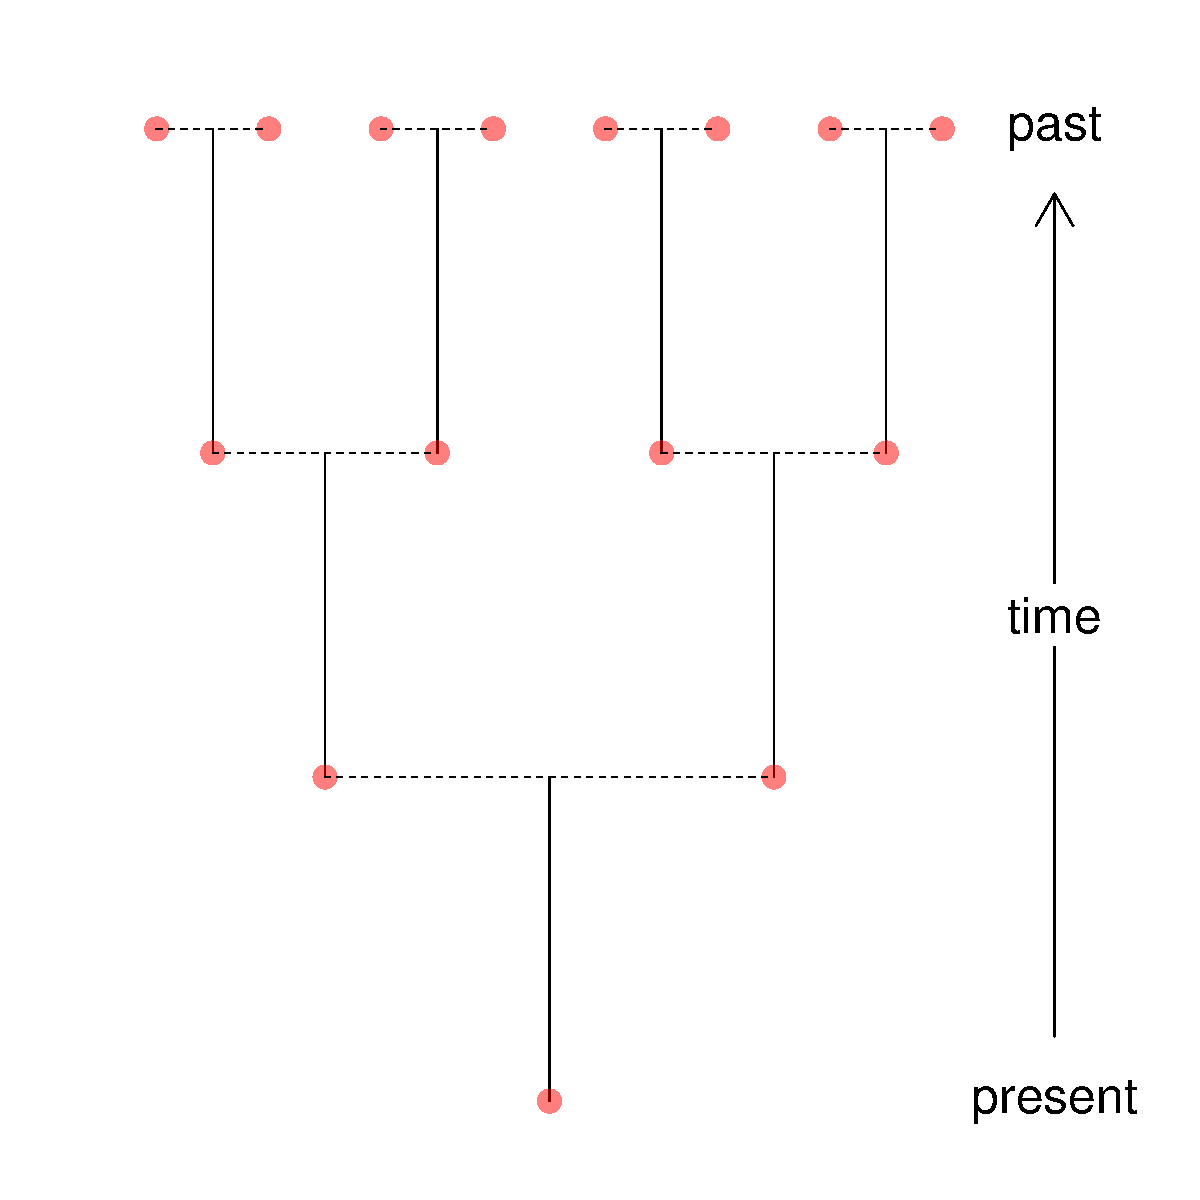
\includegraphics[width=\linewidth]{figs/pedigree.pdf}
        \caption{the pedigree}
        \label{pedigree}
    \end{subfigure}
    \begin{subfigure}{0.55\textwidth}
        \centering
        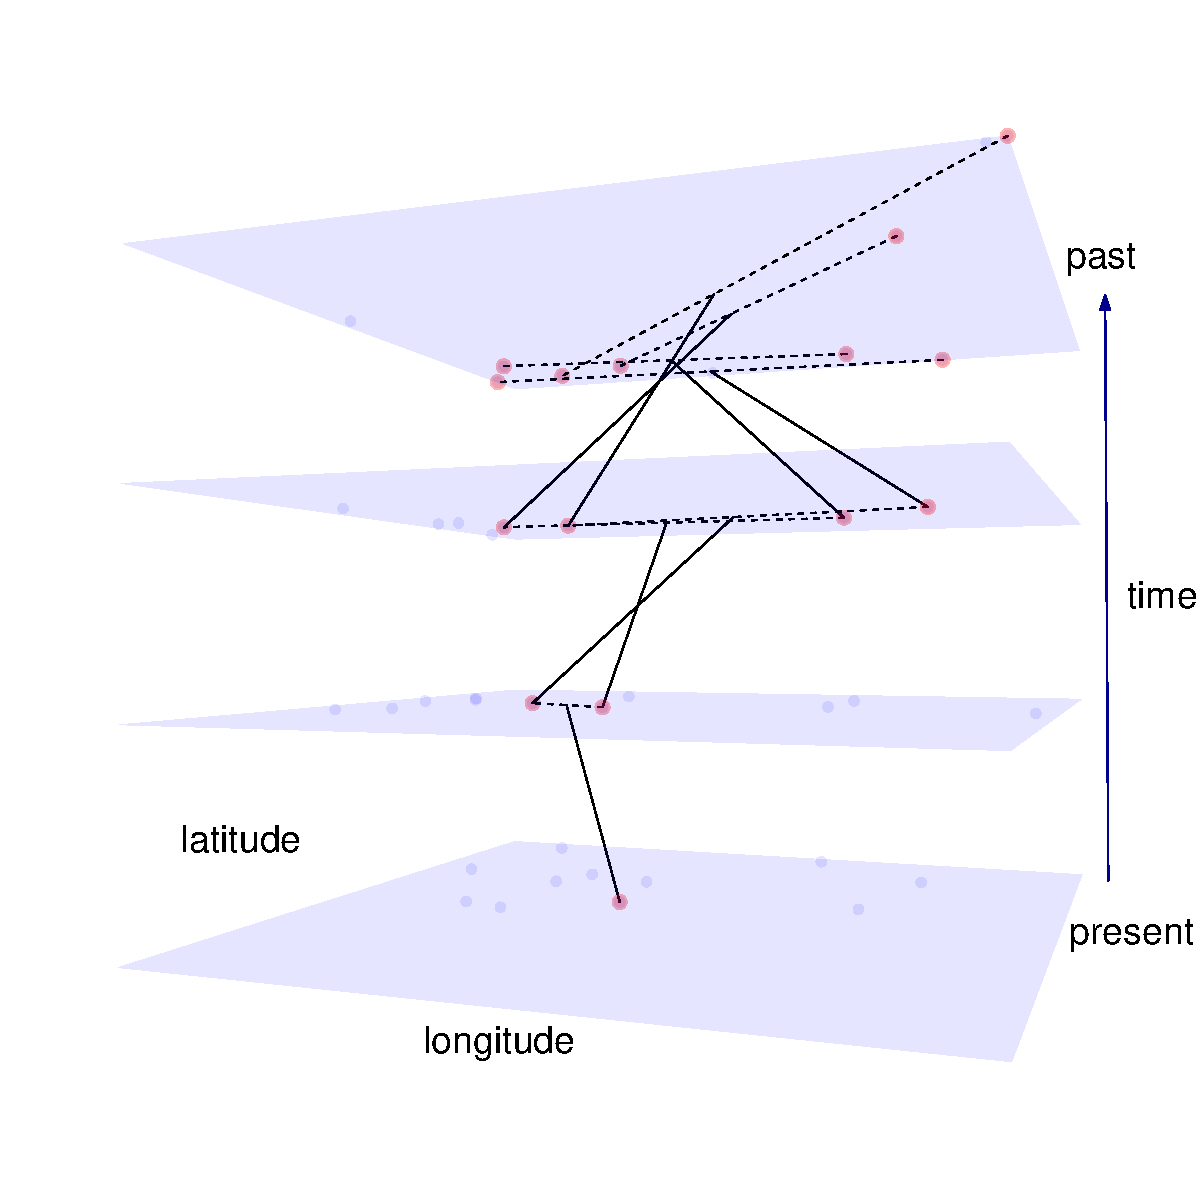
\includegraphics[width=\linewidth]{figs/spatial_pedigree.pdf}
        \caption{the spatial pedigree}
        \label{sp_pedigree}
    \end{subfigure}
        \caption{
            Example spatial pedigree.
                    Each plane represents a a sampled region in a discrete (non-overlapping generation),
                    and each dot represents an individual.
                    The present is at the bottom of the plot, and the past at the top.
                    The spatial pedigree of the ancestors of a focal individual is highlighted in red
                    back through time and across space.
                    Dashed lines denote matings, and solid lines denote parentage.
        }
        \label{spatial_pedigree}
\end{figure}

%%%%%%%%%%%%%%
\section{Things we want to know}

%%%%%%%%%%%%%%
\subsection{Where are they?}

Perhaps the first thing we want to know about a species
is their abundance and distribution:
how many are there, and where do they live?
The ideal result would be a map depicting numbers of individuals
at some level of geographic resolution.
Quantifying abundance and how it varies
can be crucial for understanding
ecologically important details of a species' natural history,
like what habitat to prioritize for conservation, 
which regions have higher population carrying capacities than others, 
or whether a particular habitat is a demographic source or sink 
\citep{pulliam1988sources,schreiber2010interactive}.
Clearly, at least some aspects of abundance and fecundity are recorded in the spatial pedigree.
%, and we can use data that were generated under this spatial pedigree
%to get a peek at the process.

%%%%%%%%%%%%%%
\subsubsection{Population density}

\todo{tidy up and tie together}

Consider a population in some geographic area. 
One quantity we would like to be able to describe 
is the average population density in a given region within that area.
What exactly do we mean by population density?
One definition is simply the total number of individuals in a given area.
However, such a count may include 
individuals who are not reproductive (e.g., juveniles), 
or those who are transient and not reproductive locally 
(e.g., born elsewhere, reproductive outside the region of interest, 
and included in a local count while passing through).
These individuals will be invisible in the pedigree 
of modern, extant individuals within the region.
Instead, we focus on the effective population density \citep{barton-depaulis-etheridge}, 
the number of individuals per unit area in a given region 
who leave ancestors in the modern day.
This quantity is analogous to effective population size \citep{wright1931evolution}
and neighborhood size \citep{Wright1943,wright1946isolation} -- 
but differs in two important aspects.
First, 
it is not associated with a discrete deme, 
but is instead defined within a specified region, 
and second, 
it may vary across different different parts of a species' range, 
and can therefore not be well summarized with a single number.
If we knew the complete spatial pedigree of a species, 
we could measure population density of an area 
by simply counting the average number of individuals born within its margins.
Without such complete knowledge, 
we must seek to estimate population density from patterns of genetic variation 
in the sample in hand.

In principle, determining population density is a very simple estimation question:
how many ancestors were there in a given region at a certain time in the past?
However, in addressing this question we quickly run into the familiar
issue of ``effective'' population size \citep{CharlesworthCharlesworthBarton2003}.
Information about population sizes in patterns of relatedness
comes from numbers of shared ancestors, i.e., \textit{coalescences}.
The reason for this is simple:
with fewer possible ancestors, the ancestors of two individuals
must be shared more often.
How likely a given individual who lived at some time in the past
is to be a genetic ancestor of a modern-day individual
is just their genetic contribution to the present population.
If we are looking one generation back, 
this is proportional to their number of offspring, i.e., their fitness.
If we are looking a long time in the past
(in practice, more than 10 or 20 generations \citep{bartonfitness}),
this is their \textit{long-term fitness}.
The effective population density we might estimate using coalescence rates
is ``effective'' partly because of this difference.

What signature does effective population density leave 
on the spatial pedigree and patterns of genetic variation
within a region?
Consider two adjacent valleys, 
one densely populated, the other sparsely populated, 
but both equal in geographic area 
and separated by a strong barrier to dispersal.
In general, we expect pairs of individuals in the low density valley 
to have shared ancestors in the more recent past than 
pairs of individuals in the densely populated valley.
To see why, consider the relationship between population density
and the pool of possible parents.
Each individual in the current generation has two parents that came from nearby,
so in the sparsely populated valley,
the pool of individuals who \textit{could} be parents gets exhausted quickly,
and individuals in the current generation
are more likely to share at an ancestor in the recent past.
Because individuals in the sparsely populated valley have more shared ancestors 
in the more recent past, 
we would expect samples from that valley to have higher probability of being identical by descent 
at a given locus, 
and for the sample as a whole to display lower heterozygosity.

However, there are a number of reasons why the genetic signature 
of effective population density may, in fact, be more complicated.
First, if dispersal distances are, on average, shorter 
in the sparsely populated valley -- 
e.g., because resources are more plentiful, 
and individuals do not have to disperse as far to avoid competition -- 
there may be more inbreeding over short distances, 
but higher heterozygosity within the valley as a whole.
In such a scenario, coalescence happens locally 
(e.g., within Wright's neighborhood size)
faster than migration connects the pedigrees of 
far-flung individuals within the valley.
Another complication is that offspring born within a particular region 
may leave and reproduce outside the region, 
which could erase their local contribution to the spatial pedigree.
Likewise, a parent of an individual within the region 
may have been born elsewhere, 
which could potentially inflate the inferred local density.
If the rates at which pedigrees enter and leave a focal area are equal, 
and density is constant, 
the pedigree permeability of the region may not affect inference of density too strongly.
However, local ecological or demographic dynamics 
can alter these rates.
For example, in a region that acts as a population ``sink,"
the rate of pedigrees entering the area is greater than 
that of pedigrees leaving the area.
An estimate of density inferred from patterns of heterozygosity 
within a sink region may be much higher than the truth, 
and the converse may hold in a ``source" region.
These dynamics are related to the concept of population ``flux" 
across a border, discussed further below.


%\todo{
%\begin{itemize}
%\item the first thing we might want to know is where everyone is
%\subitem - how many in total
%\subitem - how many per sq km here vs. there
%\subitem - what proportion in this valley vs that valley
%\item analogous to Ne, but more complicated bc it's not a single number
%\subitem - $\rho$
%\item what about pedigree tells us about pop size and or local pop density
%\subitem - just like w/ randomly mating pop, in smaller pops, you don't have to look back in time so far before you find common ancestors
%\subitem - rate of coalescence is determined by local pop density.
%\item what affects this relationship?
%\subitem  - regions of lower density should, all else being equal, have lower heterozygosity, bc heterozygosity tells you about mean(tmrca)
%but there's a lot of things that have to be equal in that statement, 
%e.g., consider 2 valleys, one large w/ low density, one large w/ high density
%should they have same heterozygosity? it depends!
%\subitem - If there's lots of isolation by distance within a valley, 
%bc sigma is smaller than the valley, 
%then coalescence will happen faster than migration.
%\item  nonreproductive individuals
%\subitem - reproductive individuals farther back in the past.  need to translate between census and effective size
%\item contrast heterogeneity in pedigree relatedness with that of genetic contributions (more in the latter than the former)
%\item Mention Fecundity and reproduction (source-sink) - note: this is flux
%\subitem - e.g., sinks are regions that are characterized by a net positive inward flux
%\item How many new offspring are produced per year in a given area? in total?
%\item How do areas contribute in the *long term*?
%\end{itemize}
%}

\begin{figure}[ht]
    \centering
    \begin{subfigure}{0.5\textwidth}
        \centering
%        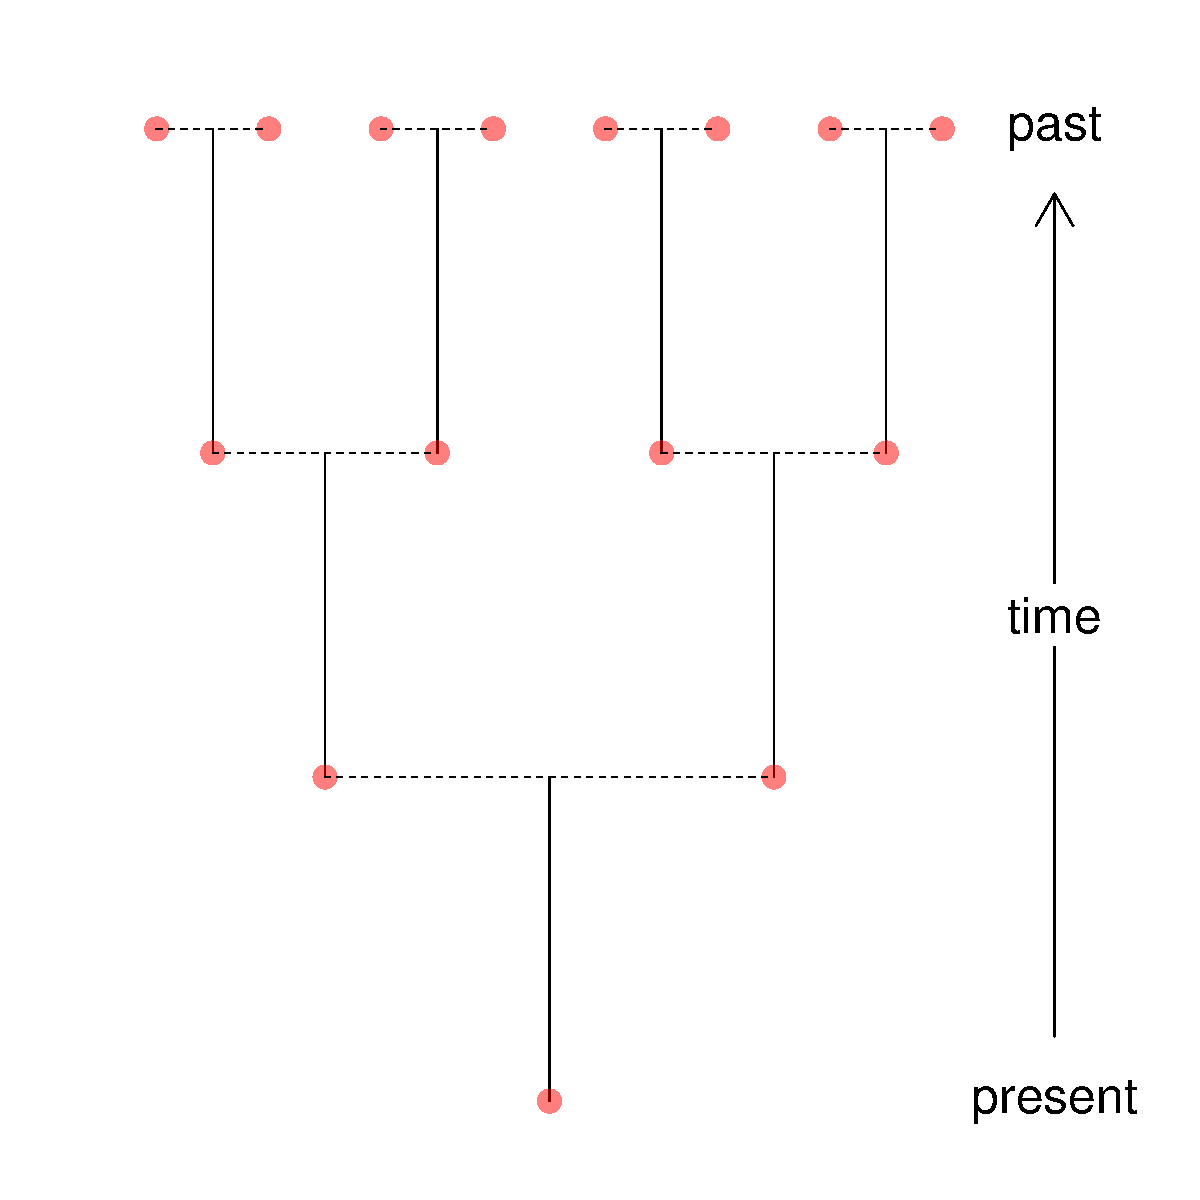
\includegraphics[width=\linewidth]{figs/pedigree.pdf}
        \caption{map of simulation scenario}
        \label{valley_map}
    \end{subfigure}
    \begin{subfigure}{0.5\textwidth}
        \centering
        \includegraphics[width=\linewidth]{figs/valley_heterozygosity}
        \caption{individual heterozygosity}
        \label{valley_het}
    \end{subfigure}
        \caption{
            \todo{map of simulation scenario (two valleys with different densities, separated by a ridge)}
            \textbf{(below)} Relative heterozygosity of a sample of 100 individuals across the range.
            Observed heterozygosities of diploids were standardized 
            by subtracting the mean and dividing by the SD;
            circle sizes are proportional to the resulting absolute value,
            and circle color indicates the sign (magenta: negative, cyan: positive).
            Low heterozygosities occur on the edges of the range,
            and average about 40\% lower in the smaller valley on the right.
		}
        \label{pop_density}
\end{figure}


%%%%%%%%%%%%%%
\subsubsection{Related statistics}

\todo{deeper coalescences in denser areas, more diversity and lower p(IBD), theta, heterozygosity, genome-sharing, drift btwn generations, or, e.g., old trees vs. saplings, patterns of LD?).
methods to mention\g{?}: Ben Peter's Ne thing, 
\cite{England2006}
estimating wright's neighborhood size (shirk, mcniel, stuff by waples)
SMC-type things
}


%%%%%%%%%%%%%%%%%%%%%%%%%%%%%%
\subsection{How do they move?}

Dispersal is fundamental to many questions in ecology and evolution,
such as
predicting responses to climate change or the spread of epidemics,
or understanding population demography and dynamics.
Organisms may move in many ways throughout their lives,
but quantities most clearly reflected in population genetic data
have to do with the displacement between geographic locations of parent and offspring
(for concreteness, taking the location of their birth or germination,
and averaging over sex of the parent).
The best overall descriptor of ``how much they move''
is often the absolute value of this displacement,
known as the between-generation \textit{dispersal distance}.

This important quantity describes how quickly spatial populations mix,
but combines many important aspects of the organism's ecology, including
any movement of gametes or zygotes before maturation,
and subsequent daily or seasonal movement of the mature individual,
all of which often depend on the sex of both parent and offspring.
For some species,
it may be feasible to directly measure many of these components
using, e.g., telemetry or banding \citep{dispersal_estimation}.
However, this is often difficult.

Furthermore, as with variation in population density,
measured dispersal of modern individuals in a handful of years
may not reflect historical averages \citep{WhitlockMcCauley1999}.
However, 
if we knew the spatial locations of ancestors in the pedigree,
then realized dispersal would be recorded directly;
we usually do not, but spatial locations of modern individuals
can give strong clues about this \citep{Cayuela2018demographic}.


%%%%%%%%%%%%%%
\subsubsection{Dispersal (individual, diffusive movement; $\sigma$)}

First, consider inference of the ``dispersal distance'',
which for the sake of discussion take as
the mean distance between the birth (germination/hatching/\textit{et cetera})
locations of a randomly chosen individual
and that of a randomly chosen one of its parents.
This notion is actually a cluster of closely related quantities:
for instance, if survival strongly depends on where an offspring disperses to,
then the ``dispersal distance'' estimated by picking an adult from the population
and measuring distance to their offspring (regardless of survival)
could differ substantially from that estimated by measuring the distance between that same adult
and \textit{her} parents.

Dispersal distance could be trivially estimated by taking
the average of these displacements across history
if we knew the spatial pedigree through time without error.
In practice, we often are only able to directly observe
the location of individuals in the present day.
However, we can still leverage this information to learn about dispersal distance,
despite not knowing parental locations, 
by comparing spatial distances between individuals of different levels of relatedness.
For example, if we sample two individuals that are siblings,
then the distance between them is the result of two dispersals,
so an average of this distance over many pairs of siblings 
gives an estimate of twice the dispersal distance.
First cousins would give four times the dispersal distance, and so forth.
The mean squared displacement between two individuals
related by a path of total length $n$ through the pedigree is $\sigma^2 n$,
assuming that $n$ is short enough that boundary effects can be ignored.
Of course, any pair of individuals are related by many paths through the pedigree,
but as in common usage we refer to this degree of relatedness
as the length of the shortest path,
and assume all other paths are much longer.
Suppose we had $K$ pairs of individuals sampled in the modern day
with known degrees of relatedness $n_1, \ldots, n_K$,
(i.e., lengths of shortest paths through the pedigree),
separated by geographic distance $x_1$ through $x_K$.
These would yield an estimate of squared dispersal distance $\sigma^2$ of
$(\sum_{i=1}^K x_i^2 / n_i^2) / (\sum_{i=1}^K 1 / n_i)$.

In practice, however, this is usually infeasible
unless a large fraction of the population has been genotyped
\citep[e.g.,][]{Aguillon2017deconstructing}.
Although long, shared tracts of genome can be used to identify very recent cousins,
these are rarely encountered in data,
and identification of more distant relatives is necessarily uncertain.
Nonetheless, how genetic relatedness decays with distance
clearly contains information about dispersal distance.
The mean squared displacement between two individuals
related by a path of total length $n$ through the pedigree
is $\sigma^2 n$,
assuming that $n$ is short enough that boundary effects can be ignored.
If, for $K$ pairs of individuals sampled in the modern day,
we had both known geographic separation $x_1$ through $x_K$
and corresponding degrees of relatedness 
(i.e., lengths of paths through the pedigree \plr{fixme})
$t_1$ through $t_k$,
then an estimate of squared dispersal distance $\sigma^2$ would be
$\frac{1}{K}\sum_{i=1}^K \|x_i\|^2 / t_i$.
%In practice... \cite{Malecot, Barton, Harald}.
%\plr{should we talk about collecting/scattering here?

This can be abstracted to any level of relatedness,
however, distinguishing more distant levels of relatedness becomes impossible,
and using longer paths through the pedigree introduces a subtle bias,
as discussed above:
individuals far back in time without descendants today
will not be included in this estimate.
\plr{discuss above}


\todo{tidy and conclude}
%It may be helpful to think of the dispersal distance
%as determining how quickly the population mixes through diffusive movement:
%local differentiation between individuals in different parts of the species range
%is determined by the balance between drift and gene flow.
%If one imagines a spatially restricted allele
%as a drop of dye in some water,
%the dispersal distance determines how quickly the
%color spreads through the water. \plr{move above?}

%Is there a mean bias (net directionality) in parent-child displacement? Anisotropy?

%Male/female differences in dispersal distance?

%%%%%%%%%%%%%%
\subsubsection{Population flux}

The most common summary statistic of dispersal in population genetics
is the average migration rate between a pair of discrete, isolated demes.
In continuous space, the analogue of this quantity
is the number of dispersal events that cross
a given boundary each year;
i.e., how many individuals are born each year whose parents
were born on the other side of a given boundary?
We call this quantity the \textit{population flux} across the boundary,
and it is a useful concept for investigating connectivity between different areas
and the role of the landscape in shaping patterns of dispersal.
For instance,
we might be interested in the flux across a ridgeline between two valleys
relative to that across a similar boundary down the middle of one of the valleys,
which can tell us whether that ridgeline is a substantial barrier to population movement or not.
Note that population flux is not constrained to be equal in both directions across a boundary;
e.g., it may be easier to disperse downhill than uphill,
downwind than upwind,
or down-current than up-current.

As before, if we had complete knowledge of the spatial pedigree,
we could calculate the flux across any line simply by counting the number of
parent-offspring pairs that span it.
In practice, we must rely on observations from genetic data,
which introduces two complications.
First, in a given dataset, it is rare to find in one individual
that is a direct ancestor of another in the dataset
(apart from perhaps some parent-child relationships).
Even with historical data (e.g., ancient DNA),
ancient individuals are unlikely to be direct genetic ancestors of modern samples,
and instead are likely to share common genetic ancestors with modern samples.
As a result, we almost never infer dispersal events,
only coalescences between pairs of individuals.
Therefore, the problem of inferring population flux from genetic or genealogical data
cannot be completely disentangled from inferring population density (discussed above).

The second complication is analogous to the problem of effective population size:
the lineages along which genetic material is passed are not an unbiased sample of all dispersal events;
they are weighted by their contribution to the population.
For instance, if there is strong local intra-specific competition,
individuals that dispersed farther from their parents (and their siblings)
may be more likely to reproduce and therefore be represented in the pedigree.
On the other hand, if there is substantial local adaptation,
then many individuals may be dispersing to habitats dissimilar to that of their parents
and are unlikely to transmit genetic material to the next generation
because they are maladapted to the local environment
(\citep[for a review, see][]{wangbradburd2014}).
With sufficient sampling,
it may be possible to get an estimate of flux in the modern sample
that is only minimally affected by these biases.
For example, it may be possible to sample maladapted individuals
before they are picked off,
or to sample individuals in a generation before reproduction.
However, in general, the difference between effective flux and actual flux
will be accentuated the farther back in time one looks.

%Effects of sampling design: suppose a big pop is next to a small pop,
%since lineages go to the big pop quickly, might need a lot of samples in the small pop
%to infer flux well.
%Also, if samples are clustered about two points,
%we won't really be able to tell if there's a barrier or not,
%since all lines we draw between the two are equivalent
%from the point of view of our samples.

\begin{figure}[ht]
    \centering
    \begin{subfigure}{\textwidth}
        \centering
        \includegraphics[width=\linewidth]{figs/valley_cousins.pdf}
        \caption{cousin map for focal individuals}
        \label{cousin_map}
    \end{subfigure}
    \begin{subfigure}{\textwidth}
        \centering
        \includegraphics[width=\linewidth]{figs/valley_ibd.pdf}
        \caption{\todo{ibd map for 4 individuals}}
        \label{ibd}
    \end{subfigure}
    \begin{subfigure}{\textwidth}
        \centering
        \includegraphics[width=\linewidth]{figs/valley_line_flux.pdf}
        \caption{flux across a valley}
        \label{valleyflux}
    \end{subfigure}
        \caption{
            \textbf{(top)} Map of close genealogical relatives of four focal individuals.
            Geographic locations of all individuals across about 25 generations are shown as small cyan dots;
            close relatives are shown as larger dots, with one color for each focal individual,
            with circle area proportional to the expected proportion of genome shared
            (i.e., $2^{-k}$, where $k$ is the number of steps in the shortest path through the pedigree to the focal individual).
            \textbf{(middle)}
            Genetic against geographic distance between each of four focal individuals (one color each)
            and 100 other individuals, from the same map as above.
            Genetic distance is calculated as expected sequence divergence.
            Two of the individuals are from the left third of the range (blue and cyan),
            and the others (magenta and yellow) are from the right third of the range.
            \textbf{(bottom)}
            Flux across two boundaries on the same continuous map as above.
            All individuals across about 8 generations are shown as small cyan dots,
            and every parent-child relationship that crosses each of the dotted lines
            is illustrated by an arrow, colored either red (if it crosses left-to-right) or blue (right-to-left).
        }
        \label{fig:dispersal}
\end{figure}

We can use these observations of coalescences to learn about the flux across a given line:
across a barrier to dispersal,
the average time to coalescence for pairs of individuals on opposite sides of the line
is longer than that between individuals on the same side.
Lower population flux means that individuals on opposite sides of a line share ancestors
less frequently.
%Also, a barrier means longer across but shorter within coal times \cite{ringbauer2018estimating}.

%relationship to dispersal: birth rate times population density times length of boundary times $\sigma/\sqrt{2\pi}$ in each direction
%if dispersal is Gaussian and boundary is straight
%If the probability of dispersing distance at least $x$ transverse to the boundary is $F(x)$,
%in a homogeneous environment with symmetric dispersal,
%and population density $\rho$,
%the number of individuals crossing the boundary
%in a particular direction
%per unit of boundary length
%is $\int_0^\infty F(x) dx$, where in the integral, $x$ denotes the distance from the boundary.
%The mean absolute distance dispersed in a particular direction
%(e.g., mean E-W displacement if barrier runs N-S)
%is $\mu = \int_0^\infty x F'(x) dx = \int_0^\infty F(x) dx$.
%If dispersal is equally likely in any direction,
%then $\mu = \E{|X|}$ where $X$ is the dispersal displacement,
%since $\sigma^2 = \E{X^2}$, if $X$ is Gaussian then...
%\plr{to fix this; this is Buffon's needle}

\todo{tidy and conclude}

%%%%%%%%%%%%%%
\subsubsection{Flux surfaces}

\todo{read through and edit}

Fluxes across lines through the landscape
describe something about population movement,
but are not as satisfying or relevant to researchers
as a map that depicts regions with greater or lesser degrees of population movement.
In heterogeneous environments,
it is clearly desirable to be able to depict local population movement 
across geography on some kind of a map.
The general description of this kind would be 
to specify for each location on the map
the probability distribution of where 
the children of a parent living at that location would end up.

To build an intuition for this,
suppose that in each small section of the map,
we recorded all the dispersal events.
We could describe this collection of dispersal events 
with the following statistics:
how far individuals go,
the mean direction they travel,
and covariance in noise about that mean.
For example, the children of a parent 
living in a long valley that follows a southwest-to-northeast axis 
and is flanked by impassable ridges might be found up-valley 
or down-valley in equal proportion, 
leading to no mean direction of dispersal, 
but a high covariance along the axis of the valley.
Alternatively, the children of a parent in an lotic environment 
might disperse more frequently down-current than up-current, 
leading to a net downstream direction of travel.

A way to summarize this by one or a few maps of scalar quantities would be to estimate, 
at each location, the mean and the covariance of the parent-offspring displacement.
The mean displacement would form a vector field over the map,
where presence of a small arrow would denote some amount of mean bias in offspring dispersal.
The covariance could be summarized by an overall mean distance and a degree of anisotropy, 
or directional dependence.
In principle, this map could be estimated using 
spatial pedigree data from only two generations 
(two generations are necessary because 
multiple combinations of mean dispersal and covariance 
could explain the spatial distribution of siblings or cousins, 
so we would need to know the parental locations).
However, in practice, it may be that 
few species are sampled with sufficient spatial density, 
or have sufficient numbers of offspring, 
to distinguish the true signal of the landscape on offspring dispersal from noise.

%low priority:
%\plr{figure idea:} vector field of ellipses and arrows
%(conceptual? from slimulation?)

%%%%%%%%%%%%%%
\subsubsection{Related statistics}

\todo{$m$ between "discrete pops", resistance distance.
methods: scat, ringbauer2018, ralphcoop, cayuela refs, cockerhaweir1993, eems, newEems, bedassle}

%%%%%%%%%%%%%%
\subsection{Where were their ancestors?}

Above, we have discussed how the dynamics of populations affect
patterns of relatedness,
i.e., how individuals reproduce and move across space.
A complementary view is to
start with individuals sampled in the present day,
then, looking backwards in time,
to ask where in space they have inherited their genomes from, 
i.e., where their ancestors lived.
This shifts perspective from moving forwards in the spatial pedigree
(past to present),
to moving backwards in time through it.
Because the signal in genetic data comes from 
shared ancestry and coalescence in the pedigree,
thinking from this reverse-time perspective 
is essential to interpreting genetic data.
However, summaries of how ancestry spreads across space 
through the pedigree can be important in their own right.
For example, humans often have a substantial interest 
in estimating the locations of their own ancestors back in time.
More generally,
we are often also interested in the partitioning of genetic diversity across space,
e.g.,
quantifying the strength of inbreeding locally,
or assessing the capacity of a population to become locally adapted.
Spatial locations of ancestry compared across sections of the genome
could also be informative about the origins and mechanisms of selective sweeps.


%%%%%%%%%%
\subsubsection{Geographic distribution of ancestry}

Consider an individual living in a population in a geographic region.
The density of the population back through time and 
dispersal distance of the ancestors in that individual's pedigree 
together determine the rate of spread of that individual's ancestry 
across space back through time.
At any point in the past,
each portion of that individual's genome can be associated 
with the ancestor from whom they inherited it.
Their genetic ancestry can therefore be apportioned across space according
to the locations of the ancestors from whom they inherited their genome.
There are a number of natural questions that arise from a description of this process.

For example, we can ask how much of an average individual's ancestry is still within a given region, at some point in the past?
How long in the past was it since a typical individual in one location had an ancestor
in another geographic region (say, the next valley over).
How far back in time do you have to go before the average proportion of ancestry that an individual inherits
from the local region they live in drops below (say) 90\%?

\todo{tidy and conclude}

\begin{figure}[ht]
    \centering
        \includegraphics[width=\linewidth]{figs/valley_ancestry_01.pdf}
        \includegraphics[width=\linewidth]{figs/valley_ancestry_20.pdf}
        \includegraphics[width=\linewidth]{figs/valley_ancestry_80.pdf}
        \includegraphics[width=\linewidth]{figs/valley_ancestry_300.pdf}
        \caption{
            Spatial locations of the ancestors of four individuals:
            at 
            \textbf{(top)} one, 
            \textbf{(middle top)}, five
            \textbf{(middle bottom)} twenty, and
            \textbf{(bottom)} seventy-five generations in the past,
            all individuals from whom the four individuals have inherited genome are denoted by a circle,
            with one color for each individual,
            and with circle area proportional to the amount of genome inherited.
            The landscape is the same as in Figure~\ref{fig:dispersal}.
            \plr{this is too many: which ones to keep?}
            \g{I say keep 1, 20, and 75.  If you go back farther, 
            	does it get even clearer that the pedigrees have ``forgotten" which side of the ridge the modern inds are on? 
		If so, that might make the point more clearly.}
        }
        \label{ancestry_spread}
\end{figure}

%%%%%%%%%%%%
\subsubsection{Geographic distribution of common ancestors}

Take a lineage, follow it back through time
the chance that lineage is in somebody historical is proportional to their long-term fitness
suppose you do that for 2 individuals,
what are the chances that those two coalesce in a particular individual
that's complicated,
but an approximation:
consider a pair of siblings - the chance that those 2 lineages coalesce in a parent of those 2 siblings could be approximated by the product of the long-term fitnesses of those siblings
and a function of the number of offspring of the parent.

\todo{tidy and conclude}
%This is neat but unclear what it means outside of human-centric whatnot.
%White/dark sands lizard example:
%if two dunes are separately colonized from dark area but little coalescence happens there
%then distribution of MRCAS could be everywhere.


%\begin{figure}[ht]
%    \centering
%    \begin{subfigure}{0.5\textwidth}
%        \centering
%%        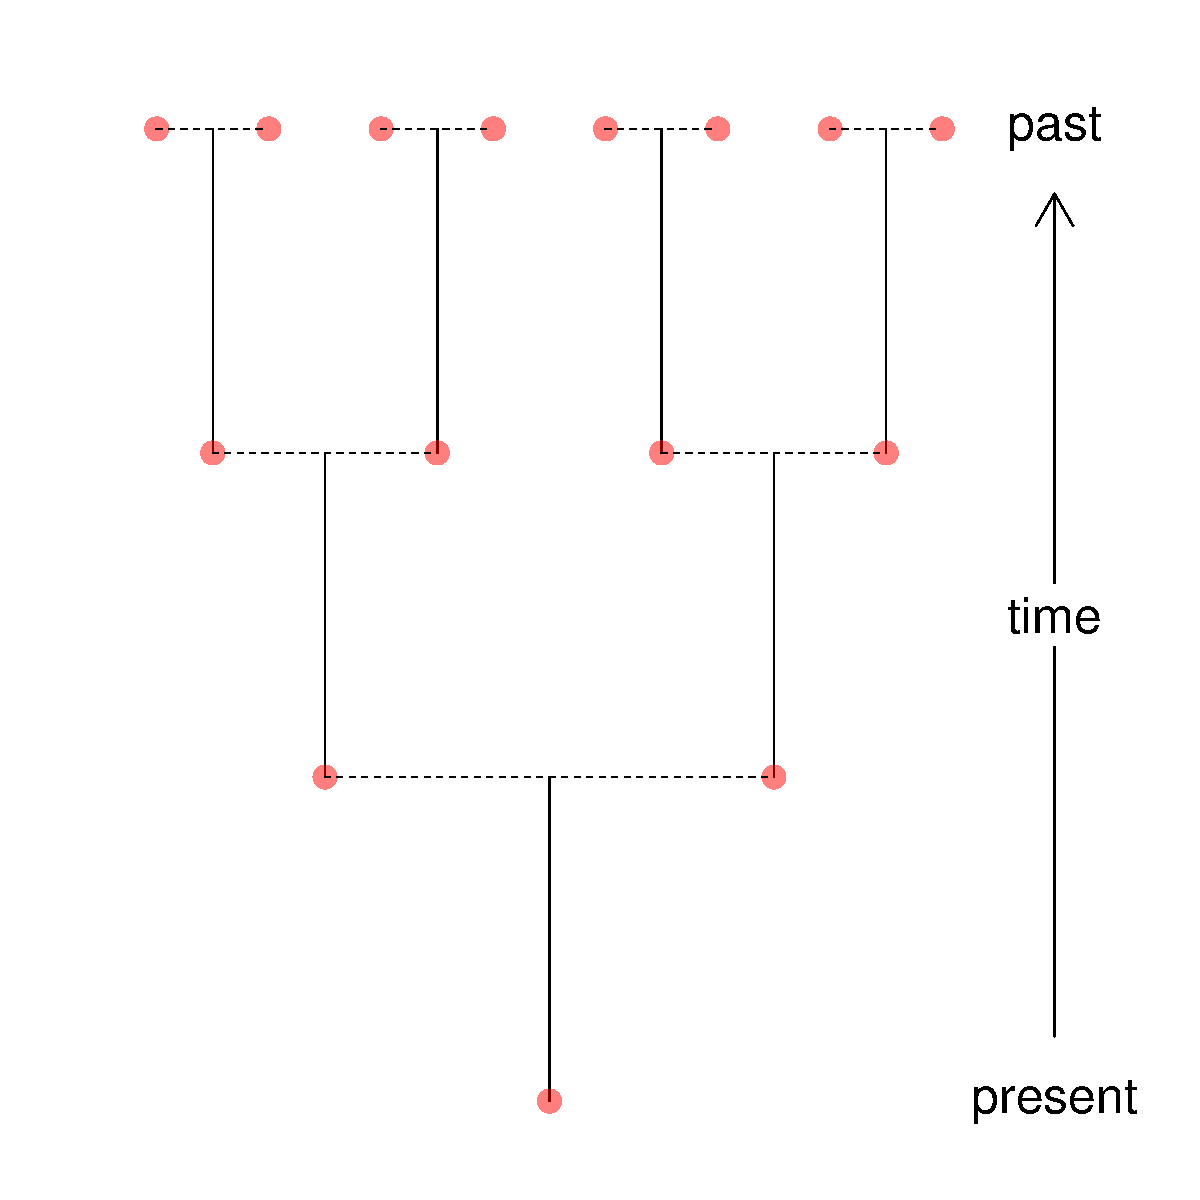
\includegraphics[width=\linewidth]{figs/pedigree.pdf}
%        \caption{nearby inds}
%        \label{nearby}
%    \end{subfigure}
%    \begin{subfigure}{0.5\textwidth}
%        \centering
%%        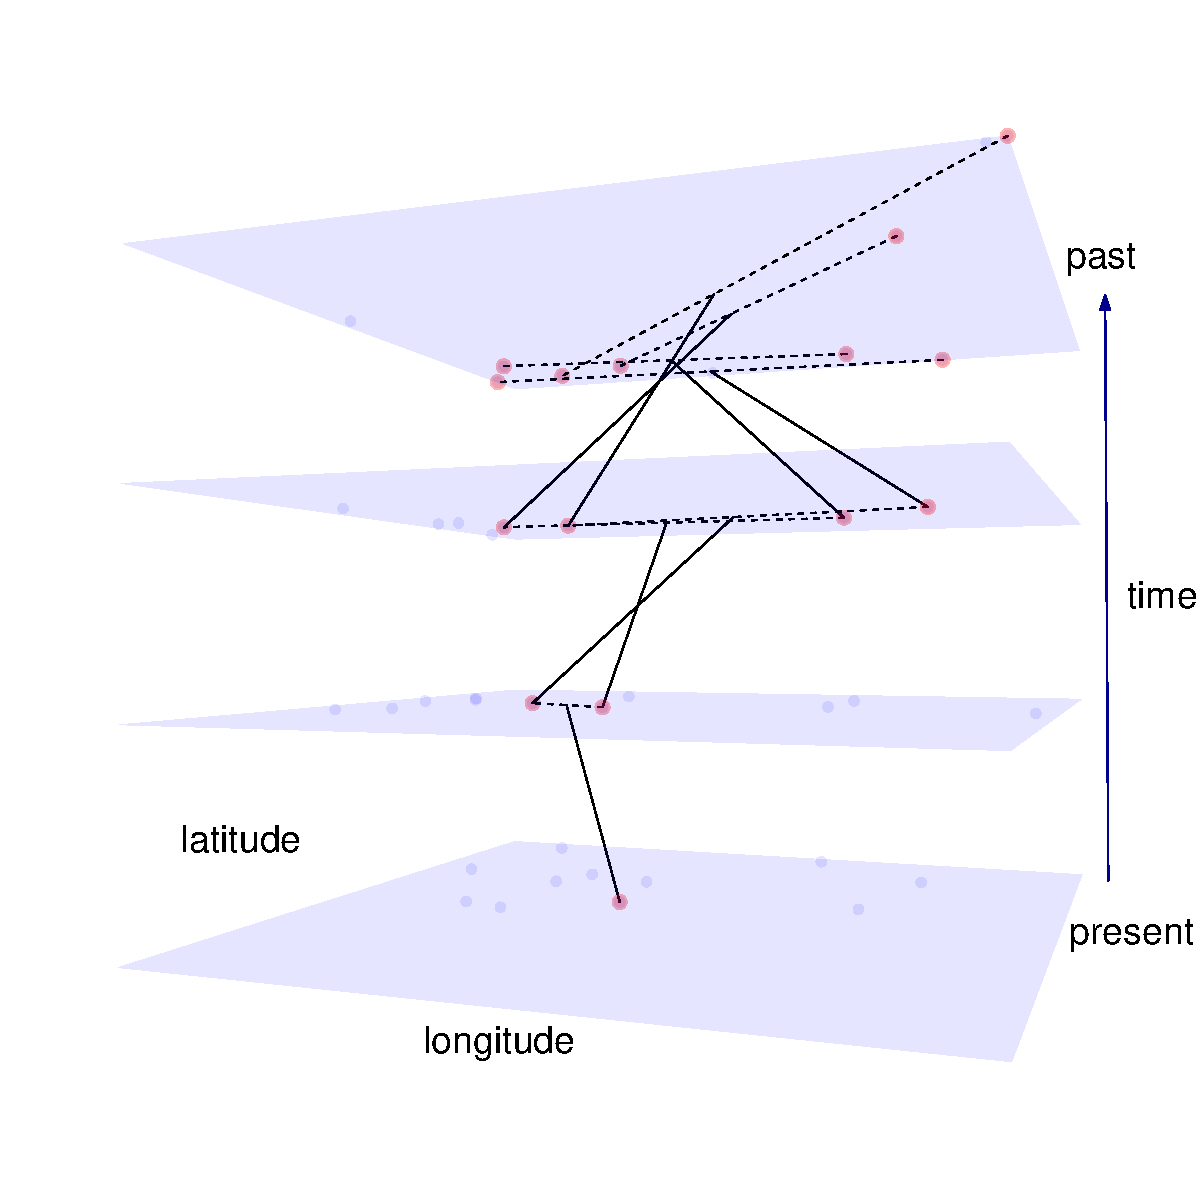
\includegraphics[width=\linewidth]{figs/spatial_pedigree.pdf}
%        \caption{distant inds}
%        \label{distant}
%    \end{subfigure}
%        \caption{
%		two maps, one for a close pair and one for a distant pair, with circles on their MRCAs
%		with size proportional to amount of genome inherited (and colored according to time?);
%		this would show the asymptote/collecting phase.
%        }
%        \label{geog_ancestors}
%\end{figure}

%%%%%%%%%%%%%%
\subsubsection{(Relative) genetic differentiation}

The question of how genetic variation is partitioned across
geography is a common and intuitively appealing one,
albeit somewhat slippery in practice.
The most common measure of this quantity is $F_{ST}$ \citep{Wright1951},
which measures how much more likely nearby individuals are to share genetic variation than individuals in the population as a whole.
Concretely,
the ratio of mean coalescence time within subpopulations
to that within the entire population measures how closely related
nearby individuals are relative to those in the entire population.
\cite{slatkin_1991inbreeding} 
showed that 1 minus this ratio is one way to interpret $F_{ST}$.
This relative genetic differentiation is determined by differing local population densities
and migration fluxes as discussed above:
relative differentiation is determined by the tension between global mixing (due to dispersal)
and local coalescence (due to small population size).
Looking at how ancestry spreads across time and space,
we can see this by looking at how quick it spreads versus coalesces.

\todo{tidy and conclude}

\g{refer to ancestry spread figure to build intuition 
for how ancestors can``forget" where their descendants are, 
leading to an asymptote in ibd}

%\begin{figure}[ht]
%    \centering
%%        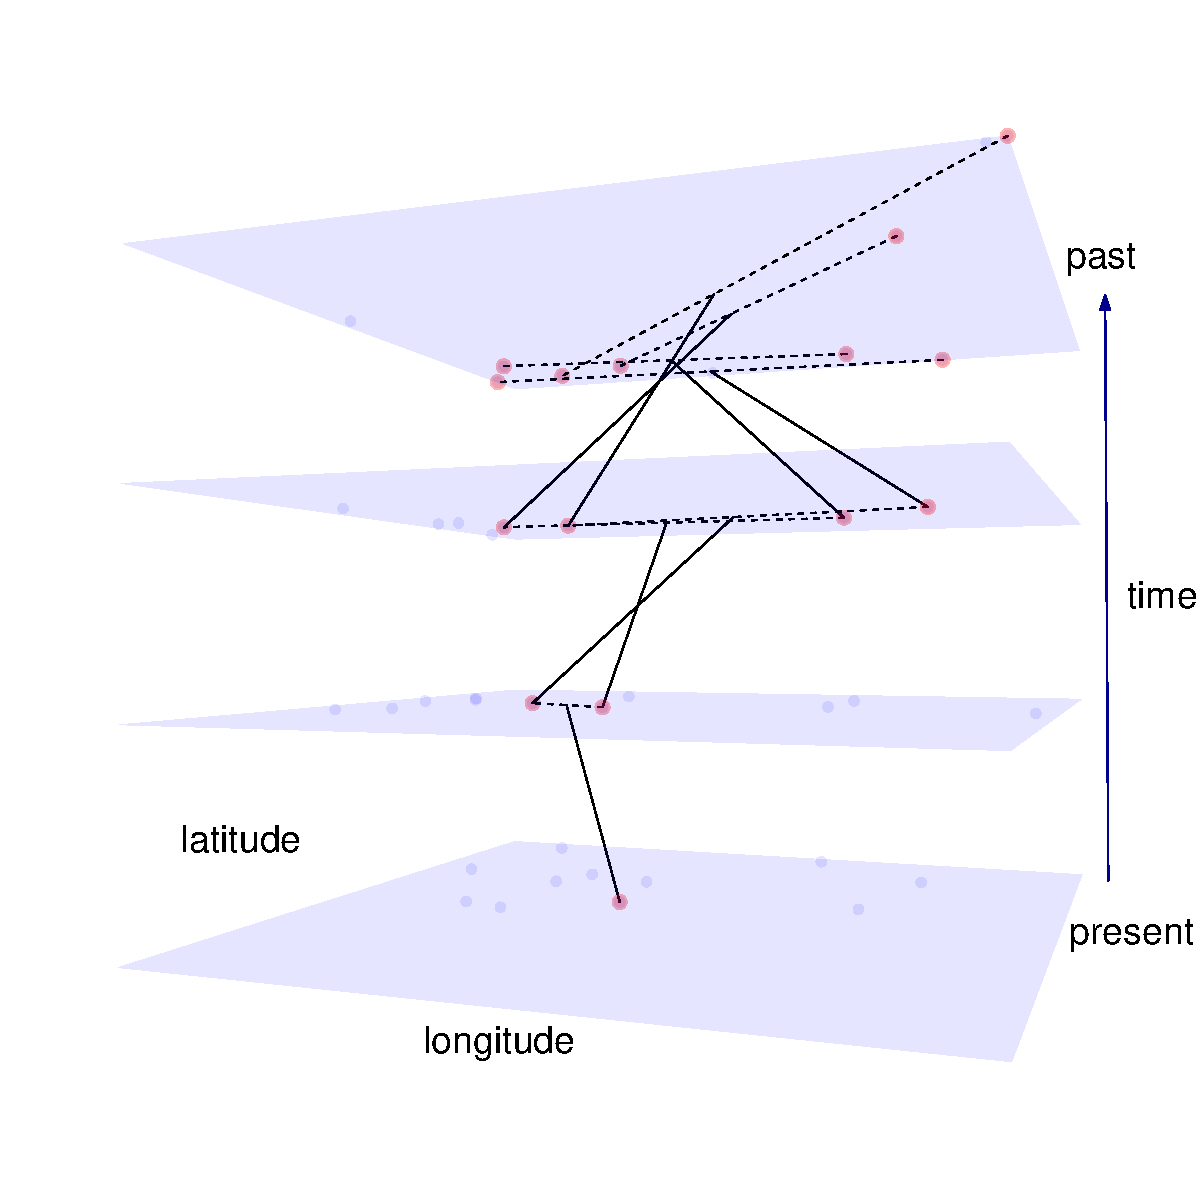
\includegraphics[width=\linewidth]{figs/spatial_pedigree.pdf}
%        \caption{
%		conceptual figure from 3.1 of tMRCA between
%		pairs of inds within each of 2 regions of different densities,
%		and between pairs of inds across the 2 regions.
%        }
%        \label{rel_gen_diff}
%\end{figure}

%
%        - How much is genetic diversity partitioned across geography?
%            How does the expected genetic divergence (or, TMRCA) for nearby individuals compared to distant ones?
%        
%            * $F_{ST}(x,y) = 1 - (\pi(x,x) + \pi(y,y))/(2 (\pi(x,x) + 2 \pi(x,y) + \pi(y,y)))$,
%                i.e., defining mean $F_{ST}$ at distance $x$ to be one minus ratio of mean TMRCA at each location
%                to mean TMRCA between individuals from the pops pooled
%
%            * relate to the classic IBD curve
%
%        - How much local inbreeding is there?
%
%            * $\pi(x,x)$? is not heterozygosity, $\pi(x,x)$ should be $\lim_{y \to x} \pi(x,y)$,
%                so we can measure this as heterozygosity minus $\pi(x,x)$
%
%refer to figure above of map of heterozygosity



%%%%%%%%%%
\subsubsection{Related statistics}

\todo{Fst, various IBD-metrics???}


%%%%%%%%%%
\subsection{How have things changed over time?}

Each of the questions discussed above --
where organisms are;
how they move;
and where their ancestors were
-- has been introduced under the assumption of a static world
where species' distributions,
the density of individuals within those species,
the dispersal patterns of those individuals,
and the landscape itself all remain constant.
In empirical systems,
these assumptions are all likely to be broken,
often drastically so.
Species are expanding into previously unoccupied territory all the time.
For example, 
high-latitude tree populations may only have been established
following the retreat of the glaciers,
a few tens of generations ago \citep{WhitlockMcCauley1999},
and invasive species may have entered their current
environment even more recently than that.
In addition to organisms moving themselves across landscapes,
landscapes are often changing out from under organisms' feet.
Anthropogenic land use change
and global climate change
are both radically altering both where organisms can live
and where they choose to
(or even where they \textit{can}) disperse.
Even within a species,
populations may show spatial discontinuity,
where most or all the ancestors of the individuals at one location
lived in another location 
\citep{bi2013unlocking,skoglund2014investigating,lazaridis_ancient_2014, joseph2018inference}.
The result of these changes is that many empirical systems
are not in equilibrium,
so that the dynamics we estimate from
measurements of extant individuals may
not be representative of those in the past.
Exacerbating this problem,
the time to reach equilibrium
in areas of high population density
or across regions of low flux
may be quite long
\citep{CrowAoki1984group, whitlock1992temporal, slatkin1993isolation, WhitlockMcCauley1999}.
Theory and methods that
reflect the empirical reality that things were not always as they are
still are lacking, 
as is a general awareness of this issue in many empirical systems.
Below we explore a few scenarios of nonequilibrium dynamics
in the spatial pedigree,
and explore how they complicate \g{inference}.

\todo{read through and edit}

%%%%%%%%%%
\subsubsection{Scenario: postglacial expansion and secondary contact}

\todo{How much does each individual inherit from each glacial refugium? Relate to admixture}

\g{to do}
\begin{figure}[ht]
    \centering
        \includegraphics[width=\linewidth]{figs/valley_admixture_new}
        \includegraphics[width=\linewidth]{figs/valley_admixture_old}
        \caption{
            Admixture proportions after a recent secondary contact.
            Each pie shows the proportion of a diploid individual's genomes
            that inherit from the left (cyan) and right (magenta) valleys, respecitvely.
            \textbf{(top)} Eight generations, and
            \textbf{(bottom)} seventy-five generations 
            after a barrier along the top of the ridge is removed.
        }
        \label{postglacial_expansion}
\end{figure}

Note also,
things change over time, e.g., if a mtn range has arisen recently, 
(e.g., orogeny induces phylogeny)
you want to look at recent flux (previous figure in reverse)

%%%%%%%%%%
\subsubsection{Now is the winter of our discontinuity}

The specter of \textit{spatial discontinuity} --
the phenomenon in which none of the individuals 
living in a particular region at a particular point in time 
are descended from any of the individuals living in that region 
at some point in the past
-- haunts the inference of historical processes in a region 
from data genotyped from extant samples.
Spatial discontinuity, 
also known as population replacement, 
can arise when regions become unoccupied
(e.g., due to ecological disturbance) 
and are recolonized by immigrants from elsewhere or 
when agonistic interactions between immigrants and local individuals 
lead to local displacement. 
Assuming that nearby individuals are more related than distant individuals, 
the genetic signature of spatial discontinuity will be most pronounced 
when the immigrant genotypes are from far away.

Spatial discontinuity presents such a problem because 
inference of many of the quantities discussed above, 
like local abundance/density, dispersal, and flux, 
is predicated on the assumption that 
the observed geographic distribution of genetic variation 
was generated in the sampled geographic context.
For example, 
we assume that the flux across the ridgeline 
depicted in Figure \ref{fig:dispersal}\subref{valleyflux}
and inferred from observed divergence 
between populations in the two adjacent valleys 
is indicative of true dispersal across the ridge.
If, alternatively, one of the valleys 
has been recently colonized by individuals from elsewhere, 
the inferred effect of the ridge on dispersal may not reflect the truth.
Spatial discontinuity in a region is especially pernicious because, 
without genotyped ancient or historical individuals, 
it may be effectively invisible.

There is abundant evidence of spatial discontinuity 
from empirical datasets that include ancient or historical samples 
\citep{bi2013unlocking, PickrellReich2014, lazaridis_ancient_2014, haak2015massive, allentoft2015population, joseph2018inference}.
And, in many systems for which we have not yet genotyped historical samples, 
we have strong reason to suspect discontinuity 
because the local populations have been recently established 
following, e.g., glacial retreat or human-mediated invasions.
As we develop more datasets that include genotype data from historical individuals, 
we will better be able to evaluate the prevalence of spatial discontinuity 
and its effects on our inferences across natural systems. 

\todo{read through and edit}
%with large-scale range shifts or population movements,
%how do you even deal?

%%%%%%%%%%%
\subsection{Are there groups of them?}
One of the most common steps in the analysis pipeline of population genetic data
is to quantify and visualize population structure:
systematic differences in genetic similarity between groups of individuals.
Perched on the shoulder of discrete population structure is the concept of admixture,
the idea that populations can be composed of ancestry from multiple discrete groups.
Models of discrete population structure and admixture 
can be helpful for getting a general sense of patterns of variation in a dataset, 
for generating hypotheses or informing future analyses, 
and, sometimes, for conservation by, 
e.g., delineating discrete management units,.
In some systems, 
especially when organisms are patchily distributed, 
with high dispersal within a patch and rare dispersal between patches,
these models may describe reality well.
However, 
the concepts of discrete population structure and admixture 
can also be a crutch that is be problematic or misleading.

All individuals within a species 
(and, indeed, across species) 
are connected via their pedigree.  
Inferred discrete population structure between groups of individuals 
relates to reduced dispersal, 
either in the modern day, at some point in the past, or both.
But, the partitioning of this pedigree into discrete groups, 
or the labeling of other samples as admixed between those groups
encourages the incorrect worldview that these populations are platonic ideals,
real and unchanging.
As has been noted elsewhere \citep{reich_india_2009,patterson_ancient_2012,hellenthal2014genetic,lawson2018tutorial},
the ability to identify a population as admixed
is a function of the recency of admixture and
the inclusion of populations descended 
from the sources of admixture in the modern day sample.
Indeed, the concept of admixture becomes slipperier when considered over deeper timescales,
as populations inferred as sources of admixture are themselves almost certainly ``admixed,"
and have either been isolated for long enough that the admixture is no longer detectable,
or, more likely, the descendants of those sources of admixture are lost in the modern sample.
Although some work has been done to incorporate models of continuous spatial differentiation 
into models of population differentiation \citep{conStruct}, 
more work is needed to acknowledge the complexity of biological reality.

\g{feel like i'm not making the point clearly}

\todo{read through, edit, rewrite?}

%%%%%%%%%%%
\section{Exciting directions for the field}

Describing the geographic distribution of genetic variation -- 
its patterns, 
the processes that have generated and maintained it, 
and its consequences -- 
is a fundamental goal of evolutionary biology.
Below, we describe a few areas 
in which we hope or expect further progress in the field to be made.

%%%%%%%%%%%
\subsubsection{Selection}
One important avenue of extension is to incorporate selection into 
models of spatially continuous populations. 
The questions introduced above are all presented in the context 
of a neutrally evolving population,
but clearly local adaptation and natural selection will impact 
the structure, and the spatial structure, of the pedigree.
Incorporating selection into spatially continuous models 
will facilitate a greater union of population genetic processes 
and ecological models of population dynamics, 
and help shed light on important evolutionary questions, 
like where adaptive sweeps originate. 
\g{more about why this is hard?}

%%%%%%%%%%%
\subsubsection{Simulation} 
A recent advance in the field, 
which may help improve inference models with and without selection, 
has been the advent of powerful and flexible simulation methods, 
such as SLiM \citep{haller2018forward,haller2018treesequence,kelleher2018efficient}.
With these methods, 
researchers can specify models of arbitrary complexity, 
and use them to simulate genome-scale datasets.
This capability offers an excellent pedagogical tool 
and opportunity to build intuition for patterns of genetic variation 
in complex scenarios for which theory may be lacking.
Indeed, we generated all figures for this paper using SLiM, 
and we have included the simulations 
and the code used to generate all figures 
as an online supplement (available for download here) 
to our paper.
In addition, these simulation methods can be used in statistical inference.
For example, simulated datasets can be used in the training 
of machine learning methods \citep[e.g.,][]{flagel2018unreasonable}, 
or to compare between different generative models using 
approximate Bayesian computation \citep{MarjoramTavare2006modern}.

%%%%%%%%%%
\subsubsection{Identifiability and ill-posedness}

Another important line of attack in developing methods for inference 
under spatial population genetic models 
is to define the limits of our ability to learn about 
quantities of interest.
For example, 
as with effective population size \citep{Myers2008},
we may never be able to infer rapid changes in 
or reversals to effective population density
\citep[although see also][]{BhaskarSong2014descartes}).
Likewise, 
the timing of heterogeneity in flux across a particular part of the landscape 
may be difficult to disentangle from the magnitude of its change, 
as is the case with migration/isolation models 
of dynamics in discrete demes \citep{sousa2011nonidentifiability}.
More generally,
it may be difficult to learn about local biases in flux, 
or large-scale anisotropy in the direction of dispersal,
without genetic data from historical individuals, 
which could be used to anchor the spatial pedigree 
in time and space.
Exploring the dependence of these quantities on each other 
using simulations and theory 
will be useful for determining what problems are well-posed, 
and what data might be most useful in solving them.


%%%%%%%%%%%
\subsubsection{The Past} 
The growing availability of genotype data from historical or ancient samples, 
collected from archaeological sites or museums 
is one of the most exciting developments in population genetics, 
and has the potential to revolutionize the field of spatial population genetics.
This historical data can provide a kind of fossil calibration on 
the alleles associated with a location in the past, 
and can also help anchor spatial pedigrees in a particular geographic context.
Although it may be unlikely that any particular genotyped historical individual 
is the genetic ancestor of any sampled extant individual, 
the geographic position of the historical sample and its 
relatedness to modern individuals is nonetheless informative 
about the geography of any focal modern individuals ancestors.
These historical data can also illuminate temporal heterogeneity 
in some of the processes described in section 3.4, 
which might otherwise be invisible in datasets comprised of only modern individuals.

%%%%%%%%%%%
\subsubsection{Conclusion}
\g{The field of spatial population genetics is the study of population genetics, in space. 
That is, the principal goals of population genetics -- 
to study patterns of genetic variation and 
learn about the processes generating those patterns 
-- are the same as those of spatial population genetics. 
However, spatial population genetics as a field 
is particularly concerned with the spatial context of these patterns, 
leveraging information in the position of samples 
to learn about processes governing 
the distribution of genetic diversity across landscapes. 
Spatial population genetics allows researchers to 
unite the quantitative descriptions of population genetics 
with fundamental questions about the ecology and evolution of organisms.}
The growing availability of genetic and genomic datasets 
with a large number of individuals and high spatial resolution, 
coupled with advances in theory and methods 
for modeling evolution in continuous space, 
is drawing us ever closer to that goal in many empirical systems.
Taken together, these developments make it 
an exciting time for spatial population genetics.



%Disclosure
\section*{DISCLOSURE STATEMENT}
If the authors have nothing to disclose, the following statement will be used: 
The authors are not aware of any affiliations, memberships, funding, or financial holdings 
that might be perceived as affecting the objectivity of this review.

% Acknowledgements
\section*{ACKNOWLEDGMENTS}
The authors gratefully acknowledge 
Graham Coop, John Novembre, 
Yaniv Brandvain, Doug Schemske, and Marjorie Weber 
for helpful feedback and discussions, 
as well as XXX, YYY, and ZZZ for invaluable comments on the manuscript.

\bibliographystyle{plainnat}
\bibliography{references}

\end{document}

%%%%%%%%%%%%%%%%
%	possible friendly reviewers: 
%%%%%%%%%%%%%%%%
Ben Peter, Nick Barton, John Novembre, 
Andy Kern, Jerome Kelleher, Josh Schraiber,
Alison Etheridge, Matthew Stephens, Kelley Harris, 
Mike Hickerson
